\documentclass[10pt]{article}

\usepackage[letterpaper, margin=1in]{geometry}
\usepackage[T1]{fontenc}
\usepackage{lmodern}
\usepackage{microtype}
\usepackage{amsmath, amssymb, amsthm}
\usepackage{booktabs}
\usepackage{multirow}
\usepackage{graphicx}
\usepackage{xcolor}
\usepackage[font=small, labelfont=bf, labelsep=colon]{caption}
\usepackage[square, authoryear, comma]{natbib}
\usepackage[colorlinks=true, linkcolor=blue!60!black, citecolor=blue!60!black, urlcolor=blue!60!black]{hyperref}

\newtheorem{proposition}{Proposition}
\newtheorem{remark}{Remark}

\newcommand{\takeaway}[1]{\noindent\textbf{#1}}
\newcommand{\x}{\ensuremath{\times}}

\title{When Does the Tensor Memory Accelerator Pay?\\
\large Reuse, Not Bandwidth, Decides: Evidence from Three Training Kernels on {H100}}

\author{Duc Bach Song\\
FPT University}

\date{November 2026}

\begin{document}

\maketitle

\begin{abstract}
Hopper GPUs add a Tensor Memory Accelerator (TMA): a copy engine in every streaming multiprocessor that moves a tile of a
tensor from global to shared memory at one thread's request, in a bank-conflict-free swizzled layout, as many stages ahead
as shared memory holds. Because TMA moves bytes no faster than threads can, its value depends on what a kernel does with
the time and registers it frees, and kernel writers have little guidance on when it is worth adopting. We rebuild three
kernels of a GPT-style training step around TMA (an AdamW update, an embedding lookup, and an \texttt{mma.sync} matrix
product), tune each over its full space of 4{,}544 to 248{,}832 settings on H100 GPUs, and check every setting bit for bit
against a reference. In the two kernels that consume each byte once, the best TMA setting runs at 0.99--1.05\x{} the plain
kernel, and TMA's two levers, the 128-byte swizzle and pipeline depth, move the time by at most 4\% in either direction.
In the matrix product, where each byte delivered to shared memory feeds 32 to 85 floating-point operations, the swizzle is
worth 1.57\x{} and depth a further 1.10\x{} over 15 products, and both win in every product. A simple bound explains the
split: on H100, shared memory has 10--13\x{} the bandwidth of HBM, more than the worst bank conflict costs, so a kernel that
reads each byte once cannot be limited by conflicts; TMA pays when data is reused.
\end{abstract}

%=====================================================================================================================
\section{Introduction}
%=====================================================================================================================

Every step of a tiled GPU kernel begins with a copy: a tile of each operand travels from global memory (HBM) into the
on-chip shared memory of a streaming multiprocessor (SM), where the threads of a block read it. Before the Hopper
architecture, the threads made that copy themselves, either through registers or, since Ampere, with the per-thread
asynchronous copy \texttt{cp.async} \citep{andersch2022hopper}. Hopper adds a dedicated unit for it, the Tensor Memory
Accelerator (TMA). One thread names a box of a tensor described by a 128-byte tensor map; the unit computes the
addresses, fills out-of-bounds elements with zeros, writes the box into shared memory in a swizzled layout, and signals
an \texttt{mbarrier} as the bytes land \citep{nvidia2022h100, nvidia2024ptx}. NVIDIA's tuning guide summarizes the
benefit as avoiding registers and SM instructions for data movement, so that the block can keep working while the data is
in flight \citep{nvidia2026hoppertuning}.

TMA does not, however, make memory faster. One block copying with TMA and four blocks copying with \texttt{cp.async} reach
nearly the same fraction of HBM3 bandwidth \citep{bose2026tma}, and each TMA copy carries a fixed latency on the order of a
hundred and seventy cycles above a plain load \citep{luo2025dissecting}. What TMA offers is a better use of the SM while the
bytes move. Whether that is worth anything depends on whether the SM has something better to do, and this, in turn, depends
on the kernel. High-performance attention and matrix-product kernels on Hopper are all built around TMA
\citep{shah2024flashattention3, spector2024thunderkittens, shankhdhar2024worklog}, but it is less clear whether a kernel
writer should reach for it in the many memory-bound kernels of a training step: optimizers, embeddings, normalizations
and element-wise operations.

This paper answers that question empirically for three kernels that sit at opposite ends of one axis, which we call
\emph{reuse}: the number of operations (and shared-memory reads) that each byte delivered to shared memory feeds before it
is discarded. Towards understanding when TMA pays, we make the following contributions:

\begin{itemize}
  \item We rebuild three kernels of a GPT-style training step around TMA, an AdamW update
        \citep{kingma2015adam, loshchilov2019adamw}, the token-and-position embedding lookup, and an \texttt{mma.sync}
        matrix product used for all 15 linear products of a 24-layer model, and tune each over its full space of settings
        on H100 GPUs (4{,}544; 32{,}800--37{,}900; and 248{,}832 per product, searched with a learned cost model). Every
        setting is checked bit for bit against a reference kernel (Section~\ref{sec:setup}).
  \item In the two kernels with reuse 1, TMA brings no speedup worth having: the best TMA setting runs at 0.99--1.05\x{}
        the plain kernel, and the swizzle and pipeline depth each change the time by 4\% or less, sometimes for the worse
        (Section~\ref{sec:streaming}).
  \item In the matrix product, the same two levers are worth 1.57\x{} (swizzle) and 1.10\x{} (depth) summed over the 15
        products, and each wins in every product (Section~\ref{sec:matmul}, Figure~\ref{fig:levers}).
  \item We give a bound in the spirit of the roofline model \citep{williams2009roofline} that predicts this split: on
        H100 the ratio of shared-memory to HBM bandwidth exceeds the cost of the worst 128-byte bank conflict, so a
        kernel that reads each byte once cannot be limited by conflicts, and its latency is hidden by occupancy rather than
        by stages (Section~\ref{sec:bound}).
  \item We check the main confounders and find that reuse is necessary but not sufficient: a CUTLASS Ampere-style kernel
        fed by \texttt{cp.async} still runs the 15 products 1.72\x{} faster than our TMA-fed \texttt{mma.sync} kernel
        (Section~\ref{sec:confounders}).
\end{itemize}

\begin{figure}[t]
  \centering
  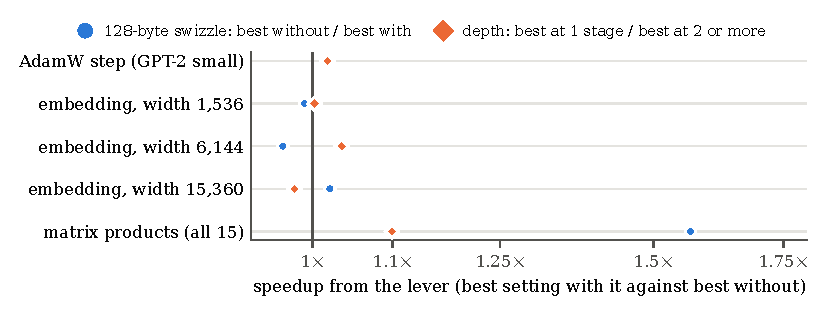
\includegraphics[width=0.92\linewidth]{fig_levers.pdf}
  \caption{TMA's two levers, kernel by kernel. Each marker is the time of the best setting without the lever divided by
  the time of the best setting with it; values right of 1\x{} mean the lever helps. The AdamW kernel copies 1-D parts and
  has no swizzle. \textbf{Takeaway:} in the kernels that read each byte once (top four rows) neither lever is worth more
  than 4\%, and neither wins consistently; in the matrix products (bottom row) the swizzle is worth 1.57\x{} and depth
  1.10\x{}. First-pass timings; H100 PCIe except AdamW (H100 SXM).}
  \label{fig:levers}
\end{figure}

%=====================================================================================================================
\section{Preliminaries and Related Works}
%=====================================================================================================================

\paragraph{Two roads into shared memory.}
With a thread copy, each of a block's threads computes the addresses of its share of a tile, checks the tensor's edges,
loads 16 bytes at a time and stores them into shared memory; \texttt{cp.async} skips the registers but still costs one
instruction and its address arithmetic per thread per 16 bytes. With TMA, one elected thread issues a single
\texttt{cp.async.bulk.tensor} instruction per box, and ``from then on address generation and data movement are handled in
hardware'' \citep{andersch2022hopper}. The consumer threads wait on an \texttt{mbarrier} whose phase completes when the
expected number of bytes has arrived \citep{nvidia2024ptx}. Because the bytes in flight occupy no registers, a kernel can
keep several \emph{stages} (tiles of future steps) in flight, limited only by shared memory.

\paragraph{Bank conflicts and the swizzle.}
Shared memory is divided into 32 banks of 4 bytes, so one 128-byte row spans every bank once
\citep{nvidia2026cudaguide}. If a tile with 128-byte rows is stored plainly, the same 16-byte column chunk of 8 consecutive
rows falls into the same 4 banks, and a read down those rows, which is the access pattern of \texttt{ldmatrix} and of the
tensor cores, is serialized 8 ways. TMA's 128-byte swizzle stores chunk $c$ of row $r$ at chunk position
$c \oplus (r \bmod 8)$, which places those 8 chunks in 8 different bank groups at no cost in space
\citep{nvidia2024ptx, colfax2024tma}. A thread copy can reach the same effect by padding each row, at the cost of extra
shared memory, or by computing the XOR itself.

\paragraph{Research on TMA, a short summary.}
Microbenchmarks place TMA's per-copy latency about 170 cycles above a plain load, show it reaching over 1{,}800 GB/s of an
H800 PCIe's 2{,}039 GB/s for large boxes, and find that boxes wide in the contiguous dimension copy faster than tall ones
\citep{luo2025dissecting}. \citet{bose2026tma} compare TMA with \texttt{cp.async} on whole workloads: TMA is faster in
319 of 324 CUTLASS matrix products (median 1.24\x{} on H100 SXM5), and in FlashAttention-3's prefill by 5.7--11.9\% in
16-bit types, but no faster in its memory-bound decode, despite issuing 26--33\x{} fewer memory instructions; below about
16~KiB in flight per SM, \texttt{cp.async} is faster. FlashAttention-3 \citep{shah2024flashattention3} builds its forward
pass on warp specialization, with producer warps that only issue TMA and consumer warps that only compute, and moves
registers from producers to consumers with \texttt{setmaxnreg}. ThunderKittens \citep{spector2024thunderkittens} wraps
TMA and \texttt{cp.async} in one load abstraction and reports a 4096-cubed matrix product rising from 260 to 760 TFLOPS as its
pipeline grows from 1 to 4 stages. \citet{shankhdhar2024worklog} documents the same path for a hand-written H100 matrix
product, where TMA, its swizzle and a circular buffer of stages are among the steps from 32 to over 600 TFLOPS. None of
these works isolates TMA's levers in kernels whose bytes are \emph{not} reused, which is where most of a training step's
kernels live.

\paragraph{Our approach.}
Rather than comparing one TMA kernel with one thread-copy kernel, we expose TMA's levers as tuning parameters and let a
sweep find the best setting with and without each lever. A lever that matters shows up as a gap between the two best
times; a lever that does not shows up as noise. We do this in kernels whose reuse differs by two orders of magnitude, on
the shapes of an actual training step.

%=====================================================================================================================
\section{Experiments}
\label{sec:experiments}
%=====================================================================================================================

\subsection{Setup}
\label{sec:setup}

\paragraph{Hardware.}
The embedding lookup and the matrix products run on an H100 PCIe (114 SMs, 2{,}039 GB/s HBM2e, CUDA 12.8); the AdamW
update runs on an H100 SXM with HBM3 (132 SMs, 3{,}352 GB/s, CUDA 13.4).

\paragraph{Kernels.}
Table~\ref{tab:kernels} summarizes the three kernels. The \emph{AdamW update} reads each weight's bfloat16 value and
gradient, its two float moments and a float master copy, and writes the updated value, moments and master back: 20 bytes
of traffic per weight for GPT-2 small's 124.4M weights \citep{radford2019gpt2}, 2{,}488.8 MB per step. The TMA version
brings a part of each tensor into shared memory per step, keeps 1 to 8 parts in flight, and writes back either through
threads or with a TMA store. The \emph{embedding lookup} computes
$\mathrm{out}[b,t,:] = \mathrm{wte}[\mathrm{token}_{b,t},:] + \mathrm{wpe}[t,:]$ for 16 sequences of 2{,}048 tokens; one
warp issues a TMA box per token row of \texttt{wte} (a gather) and one per tile of \texttt{wpe}, every thread adds its
elements in float and rounds once, and a TMA store writes the result. We run it at widths 1{,}536, 6{,}144 and 15{,}360.
The \emph{matrix product} brings each step's tiles of both operands into a ring of stages with TMA, and the warps load
fragments from shared memory and multiply with \texttt{mma.sync.m16n8k16} in bfloat16 with float accumulation. It covers
the 15 linear products of one training step of a 24-layer model of width 1{,}536 (32{,}768 tokens; QKV, attention output,
MLP up, MLP down and output head; forward, input gradient and weight gradient).

\begin{table}[t]
  \centering
  \caption{The three kernels. \emph{Reuse} is what one byte meets once it is in shared memory; for the matrix product,
  a $B_M \times B_N$ output tile performs $2B_MB_NB_K$ operations on $2(B_M+B_N)B_K$ bytes per step of $B_K$, that is
  $B_MB_N/(B_M+B_N)$ operations per byte, between 32 ($64\times64$) and 85 ($256\times128$) for the best tiles found.}
  \label{tab:kernels}
  \small
  \begin{tabular}{@{}lllrr@{}}
    \toprule
    kernel & work on one byte in shared memory & ops / byte & settings run & GPU \\
    \midrule
    AdamW update      & one update of one weight, read once            & $\approx 0.75$ & 4{,}544                     & H100 SXM  \\
    embedding lookup  & one add, read once                             & $\approx 0.17$ & 32{,}800--37{,}900          & H100 PCIe \\
    matrix product    & $B_N$ or $B_M$ multiply-adds, read by 1--8 warps & 32--85         & 11{,}904 (of 15\x248{,}832) & H100 PCIe \\
    \bottomrule
  \end{tabular}
\end{table}

\paragraph{Settings and search.}
Each kernel exposes TMA's levers as parameters next to its launch parameters (Appendix~\ref{app:spaces}). AdamW and the
embedding lookup are swept exhaustively, after removing settings whose tiles do not fit in shared memory or whose kernels
spill registers. The matrix product's space of 248{,}832 settings per product is searched with a learned cost model in the
style of AutoTVM \citep{chen2018autotvm}: a gradient-boosted ranking model \citep{chen2016xgboost} proposes 60 settings per
round and 4 more are drawn at random, after a first round of 64 random settings, and the search stops after 5 rounds
without a 0.5\% improvement. In total it ran 11{,}904 settings in 721 seconds.

\paragraph{Timing and correctness.}
Every setting is timed once in a first pass; the fastest settings are then timed again over 20 rounds, interleaved with
the plain kernel's best launch. The lever comparisons (Figures~\ref{fig:levers} and~\ref{fig:products}) use first-pass
times of the best setting in each group. Every setting's output is compared bit for bit with a reference kernel; settings
that differ are reported and excluded (none in the runs reported here; see Section~\ref{sec:confounders}).

%---------------------------------------------------------------------------------------------------------------------
\subsection{Kernels that read each byte once}
\label{sec:streaming}

Table~\ref{tab:streaming} compares the best TMA setting with the plain kernel's best launch, timed side by side.

\begin{table}[t]
  \centering
  \caption{TMA against the plain kernel in the two kernels with reuse 1, best settings timed again over 20 rounds.
  Bandwidth counts every read of \texttt{wpe} by every sequence; at width 1{,}536 both kernels exceed the HBM peak because
  L2 serves the repeated \texttt{wpe} reads (Section~\ref{sec:confounders}).}
  \label{tab:streaming}
  \small
  \begin{tabular}{@{}lrrrrr@{}}
    \toprule
    & & \multicolumn{2}{c}{plain kernel} & \multicolumn{2}{c}{best TMA setting} \\
    \cmidrule(lr){3-4} \cmidrule(l){5-6}
    kernel & bytes & ms & GB/s & ms & TMA / plain \\
    \midrule
    AdamW, GPT-2 small            & 2{,}488.8 MB & 0.8307 & 2{,}996 & 0.8423 & 0.99\x{} \\
    embedding, width 1{,}536      & 302.1 MB     & 0.1246 & 2{,}425 & 0.1241 & 1.00\x{} \\
    embedding, width 6{,}144      & 1{,}208.1 MB & 0.6058 & 1{,}994 & 0.5750 & 1.05\x{} \\
    embedding, width 15{,}360     & 3{,}020.0 MB & 1.5751 & 1{,}917 & 1.5554 & 1.01\x{} \\
    \bottomrule
  \end{tabular}
\end{table}

\takeaway{Takeaway 1.} \emph{When each byte is read once, TMA is a different way to reach the same bandwidth.} The plain
AdamW kernel already moves 89\% of the H100 SXM's peak and the best TMA setting 88\%; in the embedding lookup at width
15{,}360 the two reach 94\% and 95\% of the PCIe card's peak. Across the four cases TMA ranges from 0.99\x{} to 1.05\x{}.

\takeaway{Takeaway 2.} \emph{TMA's levers are noise at reuse 1.} Figure~\ref{fig:levers} (top four rows) and
Table~\ref{tab:levers-streaming} in Appendix~\ref{app:results} isolate the swizzle and depth. In AdamW, keeping 2 to 8 parts
in flight instead of 1 gains 1.8\%, and a TMA store instead of a thread store 2.1\%. In the embedding lookup the swizzle
is worth between 0.97\x{} and 1.02\x{} and depth between 0.98\x{} and 1.04\x{}; at width 15{,}360 the best setting uses a
single stage. A row that one thread reads once, front to back, has no conflict for the swizzle to remove, and no compute
for a deeper pipeline to hide behind.

%---------------------------------------------------------------------------------------------------------------------
\subsection{A kernel that reuses each byte}
\label{sec:matmul}

\begin{figure}[t]
  \centering
  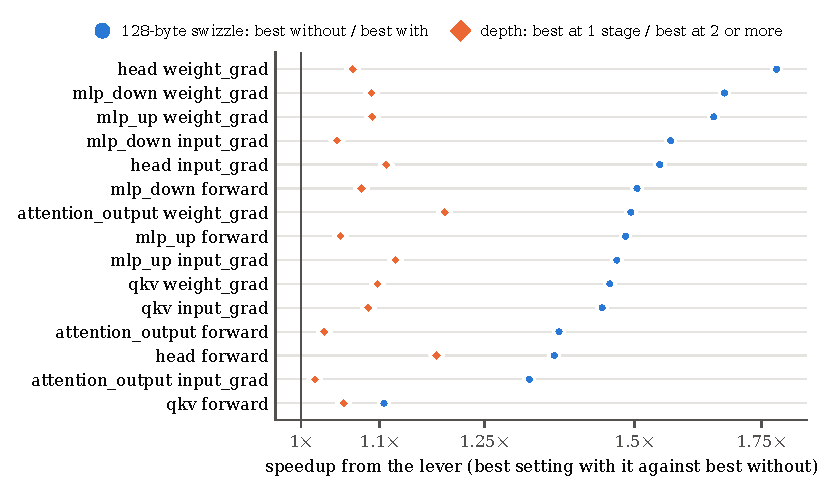
\includegraphics[width=0.92\linewidth]{fig_products.pdf}
  \caption{The same two levers in each of the 15 matrix products of one training step, sorted by the swizzle's gain. The
  swizzle wins in every product, by 1.11--1.78\x{}; depth wins in every product, by 1.02--1.19\x{}. First-pass timings,
  H100 PCIe.}
  \label{fig:products}
\end{figure}

Figure~\ref{fig:products} shows the levers product by product, and Table~\ref{tab:products} in Appendix~\ref{app:results}
gives the times. Summed over the 15 products, the best swizzled settings take 89.9 ms against 140.9 ms for the best
unswizzled ones (1.57\x{}), and the best settings with 2 or more stages take 89.9 ms against 98.8 ms with one (1.10\x{}).
The tuned kernel, re-timed, runs the 15 products in 94.9 ms against 157.6 ms at its default settings.

\takeaway{Takeaway 3.} \emph{With reuse, the swizzle is TMA's largest lever.} It is the only lever that wins in every
product by more than 10\%. The gain is largest in the three weight-gradient products with the largest outputs
(1.65--1.78\x{}), where both operands are read along the dimension TMA does not lay out as rows; we read this as more
frequent conflicts in the unswizzled layout, though we did not measure conflicts directly.

\takeaway{Takeaway 4.} \emph{Depth pays modestly and consistently.} Every product prefers 2 or more stages, most often 2
or 3. The largest gains (1.18--1.19\x{}) are in the output head's forward product and the attention output's weight
gradient; no product is fastest with a single stage.

%---------------------------------------------------------------------------------------------------------------------
\subsection{Checking for confounders}
\label{sec:confounders}

\paragraph{Run-to-run noise.}
The same launch of the plain kernels, timed in the first pass and again in the final round, differed by up to 1.0\% (for
example 0.1232 against 0.1242 ms in the embedding lookup). Differences below about 2\% in Table~\ref{tab:streaming} and
Figure~\ref{fig:levers} should therefore be read as ties. No seed-level variance applies: the kernels are deterministic and
bit-exact.

\paragraph{L2 hits in the embedding lookup.}
At width 1{,}536, both kernels report about 119\% of the HBM peak. The bytes counted include each of the 16 sequences
reading the same 6.3 MB of \texttt{wpe}, which L2 (50 MB on the H100 PCIe) serves after the first read. This reuse lives in
L2, not in shared memory, and the TMA kernel has no advantage in exploiting it: both kernels see it equally.

\paragraph{A race in an earlier run.}
An earlier sweep of the matrix product produced settings whose output differed from the reference. The cause was a race
between the threads' last reads of a stage (generic proxy) and TMA's next write to it (async proxy); a
\texttt{fence.proxy.async.shared::cta} before the barrier removes it \citep{nvidia2024ptx}, at a cost of 2--4\%. All results
reported here are from the corrected kernel, in which no setting differed from the reference.

\paragraph{TMA against \texttt{cp.async} in the matrix product.}
Our sweep compares TMA with and without its levers; it does not compare TMA with a thread copy in the same kernel. As a
reference, Table~\ref{tab:baselines} runs the same 15 products with CUTLASS's Ampere-style kernel \citep{thakkar2023cutlass}
(\texttt{mma.sync} fed by multi-stage \texttt{cp.async}, 16 tile configurations and split-K) and with cuBLAS, which uses
Hopper's warpgroup MMA.

\begin{table}[t]
  \centering
  \caption{The 15 products of one step, summed, on the same H100 PCIe. cuBLAS was timed in each run; the two timings
  are shown.}
  \label{tab:baselines}
  \small
  \begin{tabular}{@{}llrr@{}}
    \toprule
    kernel & operand path & ms & \x{} cuBLAS \\
    \midrule
    ours, default settings                 & TMA $\to$ shared $\to$ \texttt{ldmatrix} $\to$ \texttt{mma.sync} & 157.6 & 0.20 \\
    ours, tuned                            & TMA $\to$ shared $\to$ \texttt{ldmatrix} $\to$ \texttt{mma.sync} & 94.9  & 0.33 \\
    CUTLASS Sm80, tuned                    & \texttt{cp.async} $\to$ shared $\to$ \texttt{ldmatrix} $\to$ \texttt{mma.sync} & 55.2 & 0.58 \\
    cuBLAS                                 & TMA $\to$ shared $\to$ warpgroup MMA & 31.3--31.8 & 1.00 \\
    \bottomrule
  \end{tabular}
\end{table}

\takeaway{Takeaway 5.} \emph{Reuse is necessary, not sufficient.} A tuned CUTLASS kernel without TMA is 1.72\x{} faster
than ours. With \texttt{mma.sync}, every warp must still move its fragments from shared memory into registers, so the issue
slots that TMA frees are spent again on \texttt{ldmatrix}; the remaining gap lies in how warp tiles and fragment loads are
arranged, not in the global-to-shared copy. The kernels that profit most from TMA pair it with a consumer that reads
shared memory directly, and split producer and consumer warps \citep{shah2024flashattention3}; the comparison of
\citet{bose2026tma}, which holds everything else fixed, finds a median 1.24\x{} for TMA in exactly that setting.

%=====================================================================================================================
\section{Why Reuse Decides: A Bound}
\label{sec:bound}
%=====================================================================================================================

We now give a simple argument, in the spirit of the roofline model \citep{williams2009roofline}, for why the swizzle and
depth cannot matter at reuse 1 on H100, whatever the kernel.

Consider a kernel that brings $Q$ bytes from HBM into shared memory, writes each byte into shared memory once, and reads
each byte $w$ times from shared memory, each read suffering a $\kappa$-way bank conflict on average ($\kappa=1$ with no
conflicts, $\kappa\le 8$ for 16-byte accesses to 128-byte rows). Ignoring compute, its time is at least
\begin{equation}
  T \;\ge\; \max\!\left( \frac{Q}{\beta_{\mathrm{HBM}}},\; \frac{(1+\kappa w)\,Q}{\beta_{\mathrm{smem}}} \right),
  \qquad \beta_{\mathrm{smem}} = N_{\mathrm{SM}} \cdot 128\,\tfrac{\mathrm{B}}{\mathrm{cycle}} \cdot f,
  \label{eq:bound}
\end{equation}
where $\beta_{\mathrm{smem}}$ is the aggregate shared-memory bandwidth (32 banks of 4 bytes per SM per cycle
\citep{nvidia2026cudaguide}) and $f$ the SM clock. Let $\rho = \beta_{\mathrm{smem}} / \beta_{\mathrm{HBM}}$.

\begin{proposition}
\label{prop:swizzle}
If $1 + \kappa w \le \rho$, the HBM term dominates~\eqref{eq:bound}, and removing bank conflicts (setting $\kappa = 1$)
cannot lower the bound.
\end{proposition}

\begin{proof}
$(1+\kappa w)Q/\beta_{\mathrm{smem}} \le \rho Q / \beta_{\mathrm{smem}} = Q/\beta_{\mathrm{HBM}}$, and the HBM term does not
depend on $\kappa$.
\end{proof}

On the H100 PCIe ($N_{\mathrm{SM}}=114$, $f = 1.755$ GHz boost, $\beta_{\mathrm{HBM}} = 2{,}039$ GB/s), $\beta_{\mathrm{smem}}
\approx 25.6$ TB/s and $\rho \approx 12.6$; on the H100 SXM (132 SMs, 1.98 GHz, 3{,}352 GB/s), $\rho \approx 10.0$. A kernel
with $w=1$ satisfies the condition even with the worst 8-way conflict on the PCIe card ($1 + 8 = 9 \le 12.6$), and keeps
satisfying it for any clock above 1.26 GHz. This is the regime of the embedding lookup and AdamW, where the swizzle made no
difference. A matrix product is different in two ways: most of its bytes come from L2 rather than HBM (a tile is read by
every block that needs it), so the first term is small; and its compute term, which~\eqref{eq:bound} omits, is large. With
the HBM term out of the way, the shared-memory term competes only with compute, and an 8-way conflict can make it the
bottleneck, which is what the 1.11--1.78\x{} swizzle gains of Figure~\ref{fig:products} indicate. The gains stay well below
8\x{} because, once conflicts are removed, compute and fragment loads bound the kernel instead.

\begin{remark}[Depth]
By Little's law \citep{little1961proof}, sustaining $\beta_{\mathrm{HBM}}$ needs $\beta_{\mathrm{HBM}} L / N_{\mathrm{SM}}$
bytes in flight per SM, where $L$ is the memory latency; on the H100 PCIe that is $10.2 L$ bytes per SM for $L$ in cycles,
a few kilobytes for a latency of several hundred cycles. A streaming kernel reaches this with occupancy: many resident warps,
each with loads outstanding \citep{volkov2010better}. Our plain AdamW kernel launches 243{,}047 blocks of 128 threads and
our plain embedding kernel 3{,}648 blocks of 512--1{,}024 threads, and both reach 89--98\% of peak without stages. A
matrix product with large register tiles keeps only 2 to 4 blocks per SM resident, so its bytes in flight must come from
stages instead, which is why depth pays there and not in the streaming kernels.
\end{remark}

%=====================================================================================================================
\section{Conclusion}
%=====================================================================================================================

We have presented an empirical study of the Tensor Memory Accelerator in three kernels of a GPT-style training step,
tuning each over its full space of settings and isolating TMA's two levers, the swizzle and pipeline depth. In kernels that
read each byte once, TMA reaches the same bandwidth as a plain kernel and its levers are within noise; in a matrix product,
where each byte feeds tens of operations, the swizzle is worth 1.57\x{} and depth 1.10\x{}. A simple bound explains the
split: on H100 the shared-memory to HBM bandwidth ratio exceeds the cost of the worst bank conflict, so a kernel without
reuse cannot be limited by shared memory, and it hides latency with occupancy rather than stages. For kernel writers, our
recommendation is to count reuse first: adopt TMA for tiles that are read many times, and keep thread copies for
streaming kernels, where TMA adds a tensor map and a barrier for no gain.

Our findings come with some limitations. First, we compare TMA with and without its levers, and with a separately written
plain kernel, but not with a thread copy in an otherwise identical matrix product; the head-to-head comparison of
\citet{bose2026tma} covers that case. Second, our matrix product uses \texttt{mma.sync}, not warpgroup MMA, and runs at a
third of cuBLAS; the levers' sizes may differ in a kernel closer to the hardware's peak. Third, we report first-pass times
for the lever comparisons and do not measure bank conflicts or stall reasons directly; the explanation of
Section~\ref{sec:bound} is a bound, not a profile. Finally, all results are on two H100 variants; on Blackwell, where
\citet{bose2026tma} find larger TMA gains, the ratio $\rho$ and the balance between the terms of~\eqref{eq:bound} differ.

\bibliographystyle{plainnat}
\bibliography{refs}

\newpage
\appendix

%=====================================================================================================================
\section{Experimental Details}
\label{app:spaces}
%=====================================================================================================================

\paragraph{AdamW.}
5{,}120 settings: blocks per SM, threads per block (32--512), values per thread (4--32), store path (threads or TMA) and
parts in flight (1--8). 576 were skipped because they spill registers or were refused at launch; 4{,}544 ran. Model: GPT-2
small, 124{,}439{,}808 weights, a float master copy.

\paragraph{Embedding lookup.}
Blocks, warps per block (1--32), values per thread (8--128), tile rows and columns, swizzle (none or 128-byte) and sets in
flight (1--4). Settings whose tile does not fit in shared memory or whose kernel spills are removed before timing; 32{,}800,
36{,}700 and 37{,}900 settings ran at widths 1{,}536, 6{,}144 and 15{,}360. Vocabulary 32{,}768; 16 sequences of 2{,}048
tokens. An earlier sweep at width 1{,}536 over a narrower space (9{,}840 settings) gave the same conclusion (best TMA
setting 0.98\x{} the plain kernel).

\paragraph{Matrix product.}
Output tile $B_M \times B_N$ (64--256 each), step $B_K \in \{16, 32, 64\}$, 32--1{,}024 threads in a grid of warps, swizzle
(none or 128-byte), 1--8 stages, blocks per SM, and block order (1, 4, 16 or 64); 248{,}832 points per product. Settings that
need more than 255 registers per thread or spill are not built. Model: 24 layers, width 1{,}536, QKV width 4{,}608, MLP width
6{,}144, vocabulary 32{,}768, 32{,}768 tokens per step, no bias.

\paragraph{CUTLASS baseline.}
CUTLASS 2.x \texttt{Gemm} for Sm80 with \texttt{mma.sync} and multi-stage \texttt{cp.async}; 16 tile configurations
(threadblock $128$--$256 \times 128$--$256 \times 32$--$64$, warp $64\times64$, 3--5 stages) and split-K 1--8, each checked
against cuBLAS.

%=====================================================================================================================
\section{Complementary Results}
\label{app:results}
%=====================================================================================================================

\begin{table}[h]
  \centering
  \caption{TMA's levers in the kernels with reuse 1: best first-pass time (ms) in each group.}
  \label{tab:levers-streaming}
  \small
  \begin{tabular}{@{}lrrrr@{}}
    \toprule
    kernel & no swizzle & 128-byte swizzle & 1 stage & best of 2+ stages \\
    \midrule
    AdamW (TMA store)          & --- & --- & 0.8565 & 0.8412 \\
    embedding, width 1{,}536   & 0.1222 & 0.1234 & 0.1226 & 0.1222 \\
    embedding, width 6{,}144   & 0.5668 & 0.5870 & 0.5870 & 0.5668 \\
    embedding, width 15{,}360  & 1.5495 & 1.5173 & 1.5173 & 1.5495 \\
    \bottomrule
  \end{tabular}
\end{table}

\begin{table}[h]
  \centering
  \caption{The matrix products: best first-pass time (ms) with and without each lever, and the best swizzled setting's
  output tile, warp grid and stages.}
  \label{tab:products}
  \small
  \begin{tabular}{@{}lrrrrrrl@{}}
    \toprule
    product & swizzled & none & gain & 1 stage & 2+ stages & gain & best tile, warps, stages \\
    \midrule
    QKV forward                  &  2.071 &  2.291 & 1.11 &  2.182 &  2.071 & 1.05 & $64\times256$, $1\times4$, 2 \\
    QKV input grad               &  2.538 &  3.660 & 1.44 &  2.755 &  2.538 & 1.09 & $64\times256$, $1\times4$, 2 \\
    QKV weight grad              &  3.678 &  5.354 & 1.46 &  4.037 &  3.678 & 1.10 & $256\times128$, $8\times1$, 3 \\
    attention out forward        &  0.704 &  0.964 & 1.37 &  0.725 &  0.704 & 1.03 & $64\times256$, $1\times4$, 2 \\
    attention out input grad     &  0.895 &  1.181 & 1.32 &  0.910 &  0.895 & 1.02 & $64\times256$, $1\times4$, 2 \\
    attention out weight grad    &  1.426 &  2.129 & 1.49 &  1.698 &  1.426 & 1.19 & $64\times64$, $1\times2$, 2 \\
    MLP up forward               &  2.792 &  4.143 & 1.48 &  2.930 &  2.792 & 1.05 & $64\times256$, $1\times4$, 2 \\
    MLP up input grad            &  3.335 &  4.896 & 1.47 &  3.742 &  3.335 & 1.12 & $64\times256$, $1\times4$, 2 \\
    MLP up weight grad           &  4.923 &  8.131 & 1.65 &  5.368 &  4.923 & 1.09 & $128\times64$, $2\times2$, 2 \\
    MLP down forward             &  2.623 &  3.947 & 1.50 &  2.824 &  2.623 & 1.08 & $64\times256$, $1\times4$, 2 \\
    MLP down input grad          &  3.173 &  4.974 & 1.57 &  3.316 &  3.173 & 1.04 & $128\times64$, $2\times2$, 3 \\
    MLP down weight grad         &  4.984 &  8.341 & 1.67 &  5.430 &  4.984 & 1.09 & $64\times64$, $1\times2$, 2 \\
    head forward                 & 14.398 & 19.591 & 1.36 & 16.981 & 14.398 & 1.18 & $64\times256$, $1\times4$, 2 \\
    head input grad              & 17.829 & 27.581 & 1.55 & 19.783 & 17.829 & 1.11 & $128\times64$, $2\times2$, 6 \\
    head weight grad             & 24.495 & 43.668 & 1.78 & 26.091 & 24.495 & 1.07 & $128\times128$, $4\times1$, 2 \\
    \midrule
    all 15                       & 89.86 & 140.85 & 1.57 & 98.77 & 89.86 & 1.10 & \\
    \bottomrule
  \end{tabular}
\end{table}

\end{document}
